%%%%%%%%%%%%%%%%%%%%%%%%%%%%%%%%%%%%%%%%%%%%%%%%%%%%%%%%%%%%%%%%
% Christ (Deemed to be University) PhD Thesis LaTeX Template
%
% Author:Venkataswamy R
% 
% Email: venkataswamy.r@christuniversity.in
%
% Department: Electrical and Electronics Engineering
%
% Credits: Steven Gunn & Sunil Patel
%%%%%%%%%%%%%%%%%%%%%%%%%%%%%%%%%%%%%%%%%%%%%%%%%%%%%%%%%%%%%%%%
%
%  Date         |   Version   |   Author/s     | Change        |   
%  -------------------------------------------------------------
%  04-Nov-2020  |   1.0.0     |     VS         | Initial RN[1] |
%  Release Notes[1]: Created template as per the document
%  Common Guidelines for Format of PhD Thesis, V 1.1 2018
%  by Center for Research, Christ (Deemed to be University)
%
%  xx-xxx-xxxx  |   1.x.x     |     VS         | RN[2]         |
%  Release Notes[2]: 
% 
% --------------------------------------------------------------


%  Uncomment by using % symbol if you want to exlude. Do not remove
%  any line in this file.

\documentclass[12pt, oneside]{ChrisTeX} 
% All the Variable should be entered inside {}

% Research Title
\newcommand{\ResearchTitle}
{Application of Machine Leaning}

% Specialization: 
% For B.Tech : Electrical and Electronics Engineering, Mechanical Engineering 
% For M.Tech : Power Systems, VLSI Design, Software Engineering
\newcommand{\Discipline}
{Mechanical Engineering}

% Name of Research Scholar
\newcommand{\AuthorName}
{Ashok Kumar}

\newcommand{\RegisterNo}
{1RV16PEJ03}

% Gender of Author   Male/Female
\newcommand{\AuthorGender}
{Male}

% Name of the department only
\newcommand{\DepartmentName}
{Name of the department}

% Name of the College
\newcommand{\CollegeName}
{Name of the college}

% Dedication string
\newcommand{\DedicationString}
{To my beloved parents}


% Project Date in month-yyyy format
\newcommand{\SubmissionDate}
{November 2020}

% Name of the Guide
\newcommand{\GuideName}
{Name of Supervisor}

% Designation of the Guide
\newcommand{\GuideDesignation}
{Academic Designation}

% Department of Guide where he belongs to
\newcommand{\GuideDepartment}
{Name of Department}

% Name of the College where guide is affiliated to.
\newcommand{\GuideCollegeName}
{Name of the College}

\newcommand{\GuideAddress}
{Bengaluru}


% Name of the Co-Guide, if there is no Co-guide leave empty braces like {}
\newcommand{\CoGuideName}
{Name of Co-Supervisor}

% Designation of the Co-Guide
\newcommand{\CoGuideDesignation}
{Academic Designation}

% Department of Co-Guide where he belongs to
\newcommand{\CoGuideDepartment}
{Name of Department}

% Name of the College where co-guide is affiliated to.
\newcommand{\CoGuideCollegeName}
{Name of the College}


\newcommand{\CoGuideAddress}
{Bengaluru}


% Academic Year in yyyy-yyyy format
\newcommand{\AcademicYear}
{2015 to 2020}


% Name of the Director, Center for research
\newcommand{\DirectorResearchCenter}
{Name of the Director}

% Name of the RAC member 1
\newcommand{\RACMemberOne}
{Name of the RAC member 1}

% Name of the RAC member 2
\newcommand{\RACMemberTwo}
{Name of the RAC member 2}


% Date of Declaration
\newcommand{\DateofDeclaration}
{31-10-2020}

% Do not modify or delete the following lines
\hypersetup{pdftitle={\ResearchTitle}}
\hypersetup{pdfsubject=\Discipline}
\hypersetup{pdfauthor=\AuthorName}


\begin{document}

\frontmatter	
%--------------------
%	Cover Page 
%--------------------	

\makecover
	
%--------------------
%	Title Page 
%--------------------	


\maketitle

%--------------------
%	APPROVAL OF THESIS
%--------------------

\approvalofthesis

%--------------------
%	DECLARATION PAGE
%--------------------

\declaration



%--------------------
%	Certificate Page
%--------------------

\certificateguides


%--------------------
%	ACKNOWLEDGEMENTS
%--------------------

\acknowledgements{
	
	
Content here...


\begin{flushleft}
	\textbf{\AuthorName} 
\end{flushleft}

}


%--------------
%	DEDICATION
%--------------
\dedicatory{}


%-----------------
%	ABSTRACT PAGE
%-----------------

\abstract{
	
	Content... 
	
	
	\textbf{Keywords}\textit{: Keyword1, Keyword2}

}


%-----------------------------------------
%	LIST OF CONTENTS/FIGURES/TABLES PAGES
%-----------------------------------------


\tableofcontents % Write out the Table of Contents
\listoftables % Write out the List of Tables
\listoffigures % Write out the List of Figures

%----------------
%	ABBREVIATIONS
%----------------

\glossarylist{

		\begin{tabular}{lp{10cm}}
			\hline
			\textbf{Item} & \textbf{Description}\\
			\hline
			\textbf{Atomic Weight} & The atomic weight is the average of the isotope weights weighted for the isotope distribution and expressed on the $^{12}C$ scale \\
			
			\textbf{Ohms Law} & Current is proportional to voltage \\
			
			\textbf{IC Engine} & \textbf{I}nternal \textbf{C}ombustion \textbf{E}ngine \\
			
			\textbf{AIR} & \textbf{A}ir \textbf{I}ndia \textbf{R}adio \\
			
			\textbf{GUI} & \textbf{G}raphical \textbf{U}ser \textbf{I}nterface\\
			
			Speed of Light, $c$ & $2.997\ 924\ 58\times10^{8}\ \mbox{ms}^{-\mbox{s}}$ \\
			
			 $\pi$ & $= 3.14$ \\
			 
			 $P$ & Power in W (Js$^{-1}$) \\
			
			$\omega$ & Angular frequency in rads$^{-1}$ \\
			
			\hline
		\end{tabular}
		
}

%----------------
%	ABBREVIATIONS
%----------------

\abbreviations{x{4cm}p{9cm}} 
{
	\hline	
	\textbf{Abbreviations} & \textbf{Full Form of Abbreviations} \\
	\hline
	\textbf{DAQ} & \textbf{D}ata \textbf{AcQ}uisition\\
	
	\textbf{FRA} & \textbf{F}requency \textbf{R}esponse \textbf{A}nalysis \\
	\textbf{FRD} & \textbf{F}requency \textbf{R}esponse \textbf{D}ata \\
	
	\textbf{GUI} & \textbf{G}raphical \textbf{U}ser \textbf{I}nterface\\
	
	\textbf{IoT} & \textbf{I}nternet \textbf{o}f \textbf{T}hings \\
	
	\textbf{PSO} & \textbf{P}article \textbf{S}warm \textbf{O}ptimization\\
	
	\textbf{RCM} & \textbf{R}eliability \textbf{C}entered \textbf{M}aintenance \\
	
	\textbf{TOU} & \textbf{T}ime-\textbf{O}f-\textbf{U}se\\
	
	\hline
}


%----------------------------------------
%	PHYSICAL CONSTANTS/OTHER DEFINITIONS
%----------------------------------------

\listofconstants{p{3cm}x{2cm}x{1cm}p{6cm}}{
	
	\hline
	\textbf{Constant Name} & \textbf{Symbol} &  & \textbf{Constant Value (with units)} \\
	\hline
	
	Speed of Light & $c$ &  & $2.997\ 924\ 58\times10^{8}\ \mbox{ms}^{-\mbox{s}}$ \\
	
	Pi & $\pi$ & $=$ & $3.14$ \\
	\hline
	
}

%-----------
%	SYMBOLS
%-----------

\listofnomenclature{x{3cm}p{10cm}}
{
	\hline
	\textbf{Symbol} & \textbf{Description}  \\
	\hline
	$\lambda$ & Eigen Value\\
	
	$\chi$ & Cross correlation\\
	
	$\varepsilon $ & Dielectric constant\\
	\hline
}

%----------------------------
%	THESIS CONTENT - CHAPTERS
%----------------------------

\mainmatter % Begin numeric (1,2,3...) page numbering

% Chapter 1
\Chapter{INTRODUCTION}

\section{BACKGROUND}
Content...

\section{NEED OF THIS RESEARCH}
Content...

% Chapter 2
\Chapter{\uppercase{Design and Development}}

Content...

\section{Sample Figures}

\begin{figure}[h]
	\begin{center}
		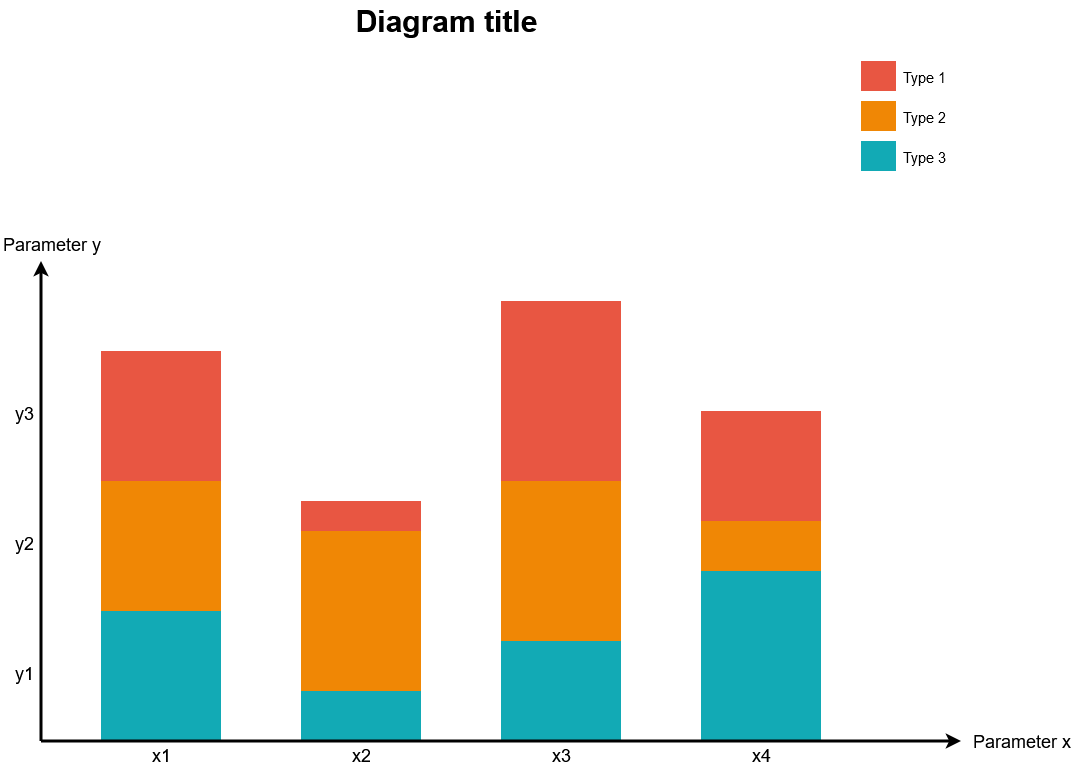
\includegraphics[scale=0.3]{Figures/bargraph.png}
		\caption{Cost distribution}
		\label{fig:costdistribution}
	\end{center}
\end{figure}

\section{Citations}

Citation \cite{Venkataswamy2020} \\
Citation \cite{Kulkarni2017} \\
Citation \cite{Venkataswamy2019} \\

Index 1 \index{Index 1}\\
Index 2 \index{Index 2}\\

\section{Sample Table}

\begin{table}[h]
	\centering
	\caption{Student Marks}
	\begin{tabular}{|r|c|}
		\hline
		\textbf{Name}  & \textbf{Marks} \\
		\hline
		Ajay  & 10 \\
		Vinay & 20 \\
		\hline
	\end{tabular}%
	\label{tab:sm}%
\end{table}%






\addtocontents{toc}{\vspace{2em}} % Add a gap in the Contents, for aesthetics

%----------------
%	BIBLIOGRAPHY
%----------------

\backmatter

\label{Bibliography}

\lhead{\emph{Bibliography}} % Change the page header to say "Bibliography"


% Option 1
%-----------------

\bibliographystyle{unsrtnat} % Use the "unsrtnat" BibTeX style for formatting the Bibliography
%
\bibliography{Bibliography} % The references (bibliography) information are stored in the file named "Bibliography.bib"


% Option 2
%-----------------

%\addtotoc{BIBLIOGRAPHY}
%
%\begin{thebibliography}{1}
%
%
%\bibitem{Sahul} 
%Hamid I. S. and Kumar S. A.  (2010), Equitable irregular edge-weighting of graphs. \textit{SUT J. Math.}, \textbf{46}, 79 - 91.
%
%\bibitem{Amar} 
%Amar D. (1993), Irregularity strength of regular graphs of large degree. Combinatorics and algorithms (Jerusalem, 1998),\textit{Discr. Math.}, \textbf{114}, no 1 - 3, 9 - 17.
%
%\bibitem{gallion} 
%Gallian J. A. (2016) , A dynamic survey of graph labeling, \textit{Electron. J. Combinator.}, \textbf{15}, 190.
%
%\bibitem{chr} 
%Chartrand G. and Lesniak (2005), Graphs and Digraphs, Fourth Edition, CRC Press, Boca Raton.
%
%\end{thebibliography}  


\publicationlist{

\begin{enumerate}
	\item Papers in Journals
	\begin{enumerate}
		\item Journal 1
		\item Journal 2
		\item Journal 3
	\end{enumerate}
	\item Paper presented in National conference
	\begin{enumerate}
		\item Conference 1
		\item Conference 2
		\item Conference 3
	\end{enumerate}
	\item Paper presented in International conferences
	\begin{enumerate}
		\item International Conference 1
		\item International Conference 2
		\item International Conference 3
	\end{enumerate}
\end{enumerate}

}

%--------------------------------
%	THESIS CONTENT - APPENDICES
%--------------------------------

\addtocontents{toc}{\vspace{2em}} 

\appendix 

% Appendix A
\chapter{Appendix A. Title}

Content...
% Appendix B

\chapter{Appendix B. Title} 


Content...






%--------------
%	Index Page
%--------------
\printindex

\end{document}  


% ---------------------------------------------------------------
% Licence: GNU GPL v3											
% This program is free software; you can redistribute it and/or
% modify it under the terms of the GNU General Public License
% as published by the Free Software Foundation; either version 3
% of the License, or (at your option) any later version.
%----------------------------------------------------------------